\mysection{The Knave}{trope-knave}


  \flavor{Fortune and glory, kid. Fortune and glory. \Tilde Indiana Jones}

\begin{center}
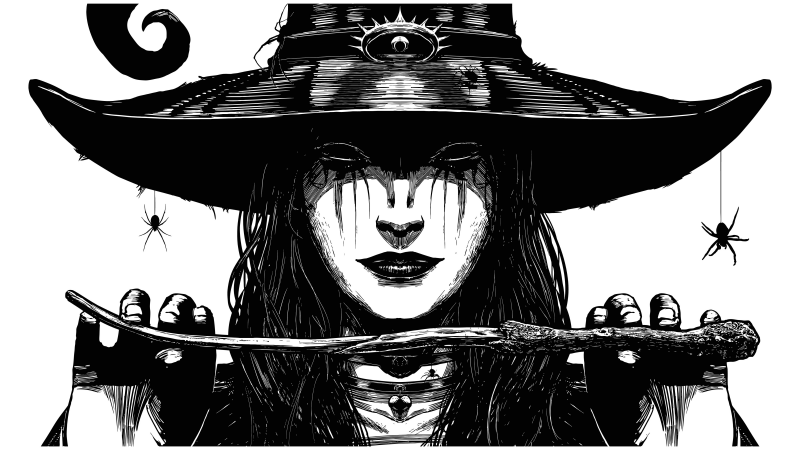
\includegraphics[width=\linewidth,keepaspectratio=true]{tropes/Knave1}
\end{center}


   \mysubsection{Creation}{knave-creation}

  Write down the following information on your \mylink{Adventurer Sheet}{adventurer-sheet.3}.
  
  \callout {
    \mynumlist {
        \item You start with \mybold{4 Flesh and 6 Grit}.
        \item Move your \DEX~ \DCUP (to a d10). Pick \VIG, \INT, or \FOC and move it \DCDOWN (to a d6).
        \item If you need to \RSTRY{\DEX}, you only fail on a natural 1 (instead of a 1 or 2). Put a check next to \DEX on your Adventurer Sheet so you don't forget.
        \item You have a d4 \mylink{Lucky Die}{knave-lucky-die}.
        \item You have all 4 \mylink{Whispers}{knave-vulgate-whispers} at a rank of Untrained (1) (see below).
        \item Choose three different \mylink{Virtues}{knave-virtues} and one \mylink{Complication}{knave-complications}. Modify your sheet as necessary.
        \item Write down your \mylink{Starting Gear}{knave-starting-gear}.
    }
 }

\newpage
\begin{multicols*}{2}\raggedcolumns

  \myhighlight{Lucky Die}{knave-lucky-die}

  Your Lucky Die is a Resource Die whose result can be applied to \mybold{any} \RO or \RB try you make \mybold{outside of} \mylink{Combat}{combat}. 

  Additionally, you may roll your Lucky Die and add its result to any \mylink{Whisper}{vulgate-whispers} try (in or out of Combat). You can only gain a maximum of +4 to your Whisper try. You can roll your Lucky Die \myital{after} you roll your try (it doesn't have to be at the same time), but you can only roll your Lucky Die once per Moment or Whisper try. 

\mybold{Your Lucky Die starts as \UDD{d4}}. Your Lucky Die moves \DCDOWN on Failure.


  \myhighlight{The Whispers}{knave-vulgate-whispers}

  Sleight-of-hand; minor glamours and illusions; telekinesis; body and mind mastery; escape artistry; mind-tricks; machine linguistics - the \mypg{Vulgate of Whispers}{vulgate-whispers} or the "Left Hand Path" allows you to alter reality without needing to meddle in the Chaos of the \mylink{Arcana}{arcana}.

\mybold{You start with a rank of Untrained (+0) in all 4 Whispers:} 
    \mybullet {
        \item the \mylink{Whispers of Anne Bonney}{vulgate-whisper-anne-bonny}, 
        \item the \mylink{Whispers of Br'er Rabbit}{vulgate-whisper-brer-rabbit}, 
        \item the \mylink{Whispers of Sun Wukong}{vulgate-whisper-sun-wukong}, and 
        \item the \mylink{Whispers of the Bride}{vulgate-whisper-the-bride}. 
    }

Note that even if you're Untrained, you have the ability to cast spells from Fetishes (\mylink{Whispers of Br'er rabbit}{vulgate-whisper-brer-rabbit}) and the ability to \mylink{Murder}{vulgate-whispers-murder} someone.


  \myhighlight{Mortal}{knave-mortal}
    
  You are creature of Order, and possess a soul - and are thus \mybold{Hallowed}.

    \cbreak

  \mysubsection{Starting Knave Virtues}{knave-virtues}

    \begin{center}
        \myemph{Choose 3 of the following}
    \end{center}


    \myhighlight{Charms}{knave-virtue-charms}

    You can perform the \mypg{Vulgate of Charms}{vulgate-charms} at will.


    \myhighlight{Deadeye}{knave-virtue-deadeye}

    In addition to the weapons specified under \mypg{Murder}{vulgate-whispers-murder}, you may also use a \DEX~ Throw or Shoot weapon to do your killing. You must still have \mypg{the Drop}{combat-drop} on your victims.

    \myhighlight{Guilded}{knave-virtue-guilded}

    You are the ex member of a Thieves' Guild (tell the Arbiter the name of your ex-Guild, and why you left). In addition to your \mylink{Starting Gear}{knave-starting-gear}, pick up to \mybold{three} items from the following list:
    \callout {
      \footnotesize {
      \mybullet {
        \item a suit of \mylink{Light Armor}{gear-armor};
        \item a set of two silver \mylink{Daggers}{gear-dex-weapons};
        \item a \mylink{Bow}{gear-dex-weapons} and a \mylink{Quiver of Arrows}{gear-equipment};
        \item 5 picks from the \mylink{Tools}{gear-equipment} table;
        \item a pouch of 3 gems (roll on the \mylink{Gems table}{appendix-a-gems} in Appendix A);
        \item \UDD{d4} of a \mylink{Narcotic}{gear-narcotics} of your choice;
        \item a \mypg{Fetish}{fetishes} with \UDD{d4} of any \mypg{Secret}{arcana-wizardry-secrets} you choose;
        \item \UDD{d4} of an \mypg{Noxious (d6) Toxin}{malignants-toxins}
      }
      }
    }


    \myhighlight{Hard to Kill}{knave-virtue-hard-to-kill}

    You're tougher than most. Gain +2 Flesh and +2 Grit. Your \DEATH moves \DCUP to \mybold{Tough (d4)}. 

    \newpage

    \myhighlight{Inked}{knave-virtue-inked}

    You start the game with the following \mypg{Tattoos}{research-inscription-tattoo}:  Dagger, Torch, Compass, and Rope.


    \myhighlight{Medicine}{knave-virtue-medicine}

    You can perform the \mypg{Vulgate of Medicine}{vulgate-medicine} during \mypg{Downtime}{downtime-shopping}.


    \myhighlight{Mummy's Curse}{knave-virtue-mummys-curse}

    If you carry or wear cursed or supernatural items, you are immune to their effects provided you intend to sell the item and don't benefit from it directly. If you decide to keep the item or benefit from it in any (non-financial) way, the curse immediately takes effect (though you still get a Save). You can’t give the item to someone else without first receiving something of value (Arbiter's discretion) in return - failure to do so means the curse immediately takes effect (though you still get a Save). Finally, if the item remains unsold before you take Downtime at a Settlement, you must sell it during the Shopping Step or the curse immediately takes effect (though you still get a Save).

    \myhighlight{Sacraments}{knave-virtue-vulgate-sacraments}
   
    You gain a single Grace die (d4) which allows you to perform the \mypg{Vulgate of Sacraments}{vulgate-sacraments}.


    \myhighlight{Whispers of Anne Bonny}{knave-virtue-anne-bonny}

    You are an Apprentice (d4) in the Whispers of Anne Bonny, a swashbuckler who can climb unscalable walls, disguise yourself, forge documents, and swing from chandeliers and ropes.

    \myhighlight{Whispers of Br'er Rabbit}{knave-virtue-brer-rabbit}

    You are an Apprentice (d4) in the Whispers of Bre'r Rabbit, a novice in the craft of picking pockets, escaping capture, performing sleight-of-hand, and casting Mysteries from \mypg{Fetishes}{fetishes}.


\cbreak

    \myhighlight{Whispers of Sun Wukong}{knave-virtue-sun-wukong}

    You are an Apprentice (d4) in the Whispers of Sun Wukong, skilled in the manners of hiding things on your person, finding and disarming traps, and opening locks.


    \myhighlight{Whispers of The Bride}{knave-virtue-the-bride}

    You are an Apprentice (d4) in the Whispers of The Bride, a student in the arts of moving silently, hiding in shadows, and \mypg{Murder}{vulgate-whispers-murder}.


\myimage{tropes/Knave2}
 
\mysubsection{Knave Complications}{knave-complications}

    \begin{center}
        \myemph{Choose 1 of the following}
    \end{center}




    \myhighlight{Arch-Nemesis}{knave-complication-archnemesis}
    
    You have an arch-nemesis who always seems to be a step ahead of you when it comes to obtaining artifacts. Tell the Arbiter a little bit about them.

    \myhighlight{Cursed}{knave-complication-cursed}

    Probably should have left that amulet alone. Roll on the \mypg{Lesser Curses table}{table-lesser-curses} - you start the game under that curse. Tell the Arbiter how you acquired this curse.

    \myhighlight{Expensive Tastes}{knave-complication-tastes}

    You have exquisite and deviant tastes for the finer things in life. It costs you twice as much to take the \mylink{The Shopping Step}{downtime-shopping} of \mylink{Downtime}{downtime}.

    \myhighlight{Honor Among Thieves}{knave-complication-honor}

    You're a professional, and you appreciate other professionals. You'll always give a hand to a fellow Knave even if that might inconvenience you or your \mylink{Band}{roles-band}.

    \myhighlight{Outstanding Contract}{knave-complication-contract}

    There's an outstanding contract on your head, revenge for something you did. Tell the Arbiter who is after you and why they want to kill you.

    \myhighlight{Pacifist}{knave-complication-pacifist}

    You won't ever start a fight (including stabbing someone unawares in the back). You have no problems fighting once a fight is joined, however. 


    \myhighlight{Pandemonium}{knave-complication-pandemonium}

    You spend money as fast as you can make it, steal from the rich to give to the poor, and thrive in chaos. You aren't motivated by anything material; you want anarchy, discord, and confusion.  


    \myhighlight{Religious}{knave-complication-religious}

    You are very religious (secretly or not). You don't worship a specific Small God necessarily, but you have enormous respect for Mystics, \TheAuthority, and the Authorities. You won't steal anything from a church or temple; priest of priestess - regardless of the Small God.

\cbreak

    \myhighlight{Remorseless}{knave-complication-remorseless}

    You feel nothing when you take a life or cause pain, but you suffer from \mypg{Night Terrors}{injury-insanity-madness}. This affliction can never be cured.


    \myhighlight{Superstitious}{knave-complication-superstitious}

    You are extremely superstitious (and believe this superstition has kept you alive up until now). You prefer the company of \mylink{Pooka}{species-pooka} whenever possible. You won't steal from the dead, or take anything from tombs or graves.


  \mysubsection{Starting Gear}{knave-starting-gear}

    In addition to any gear you might have gained from Virtues, you have:

  \callout {
    \footnotesize {
      \mybullet {
        \item 8 iron pieces; 
        \item a worn bedroll;
        \item a set of belt pouches;
        \item \UDD{d4} of \mylink{Personal Provisions}{gear-equipment};
        \item two iron \mylink{Daggers}{gear-dex-weapons} OR one \mylink{Short Sword}{gear-dex-weapons};
        \item one pick OR 3 rolls on the \mylink{Random Items}{appendix-a-random-items} table in Appendix A
      }
    }
  }

  
    \myhighlight{What Next?}{knave-what-next}

    Knaves use the \mypg{Vulgate of Whispers}{vulgate-whispers} for most of their skills; having a good understanding of them will be crucial. If you're playing an assassin / back-stabby type of Knave, read up on the rules for \mylink{the Drop}{combat-drop} under \mypg{Combat}{combat}, and \mylink{Murder}{vulgate-whispers-murder} under \mypg{Whispers of The Bride}{vulgate-whisper-the-bride}.

\end{multicols*}

